\documentclass{article}
\usepackage{graphicx}
\usepackage{amsmath}
\usepackage{amssymb}
\usepackage{natbib}
\renewcommand{\refname}{References}
\usepackage{url}

\title{On Trading of ETFs based on the Differential Geometric Forecast Model}

\author{Babak Emami}

\date{\today}

\begin{document}
\maketitle

\begin{abstract}


\end{abstract}

\section{Introduction}\label{section:introduction}

Here we propose two approaches for trading of exchanged-traded
funds (ETFs) based on the differential geometric economic forecast
model. The reader should refer to the notes on this model for details.

\section{Approach I: Maximize Predicted Return}\label{section:approach-1}

The first proposed approach is based on maximization of predicted
portfolio value growth normalized by standard deviation of prediction,
that is the risk associated with forecast. This approach is in theory
reasonable. However, as will be shown, this approach does not work
because the model is not accurate enough. As we improve the model,
this approach may become relevant.

At any given current time $t_{0}$ we build a differential geometric
model based on historical data. The model consists of $n$ economic
variable including $\tilde{n}$ ETFs that we plan to use for trading.

The model provides us with a system of ODEs; given the current values
of the model's $n$ economic variables as initial conditions, the
solution of these ODEs yields forecast of economic variables.

Let us assume that we entered $q_{i}$ positions of asset $i$ at time
$t_{0}$; the values are posive and negative for long and short
positions, respectively. The predicted value of our portfolio at time
$t$ > $t_{0}$, that is $V(t)$ is calculated as,

\begin{equation}\label{eqn:prt-value}
V(t) = \sum_{i=1}^{\tilde{n}} q_{i} y^{i}(t)
\end{equation}

where $y^{i}(t)$ is predicted price of asset $i$ at time $t$. 

Note that we consider $y^{i}(t)$ a random variable with an expected
value of $\bar{y}^{i}(t)$ and a standard deviation of $\sigma^{i}$ (it
is not a function of time). The expected portfolio value is calculated
as

\begin{equation}\label{eqn:expected-prt-value}
\bar{V}(t) = \sum_{i=1}^{\tilde{n}} q_{i} \bar{y}^{i}(t)
\end{equation}

The variance of $V(t)$ is calculated as

\begin{equation}\label{eqn:stdev-prt-value}
VAR[V(t)] = \sum_{i=1}^{\tilde{n}} q_{i}^{2} (\sigma^{i})^{2}
\end{equation}

We determine the asset quantities $q_{i}$ by solving the following
optimization problem,

\begin{equation}\label{eqn:optimization-problem-V}
\max_{q_{i}} \frac{\bar{V}(t_{H})-V(t_{0})}{VAR[V(t_{H})-V(t_{0})]}
\end{equation}

Using Eqs.~\ref{eqn:expected-prt-value} and \ref{eqn:stdev-prt-value},
we get

\begin{equation}\label{eqn:optimization-problem-q}
\max_{q_{i}} \frac{\sum_{i=1}^{\tilde{n}}
  q_{i} [\bar{y}^{i}(t_{H})-y^{i}(t_{0})]}{(\sum_{i=1}^{\tilde{n}}
    q_{i}^{2} (\sigma^{i})^{2})^{1/2}}
\end{equation}

where $t_{H} > t_{0}$ is the end of our trading horizon. In other
words, we plan to adjust our portfolio again at $t{H}$, or more
generally every $t_{H}-t{0}$.

When solving \ref{eqn:optimization-problem-q}, we should consider that
values of $q^{i}$ can be only integers. A simpler approach is to
convert quantities to portfolio weights; $w_{i} = \frac{q_{i}
  y^{i}(t_{0})}{V(t_{0})}$. The optimization probelm become,

\begin{equation}\label{eqn:optimization-problem-w}
\max_{w_{i}} \frac{\sum_{i=1}^{\tilde{n}}
  w_{i} r^{i}(t_{H})}{(\sum_{i=1}^{\tilde{n}}
  w_{i}^{2} (\frac{\sigma^{i}}{y^{i}(t_{0})})^{2})^{1/2}}
\end{equation}

subject to the following equality constraint,

\begin{equation}\label{eqn:sum-constraint}
\sum_{i=1}^{\tilde{n}} |w_{i}| = 1
\end{equation}

where $r^{i}(t) = \frac{\bar{y}^{i}(t)-y^{i}(t_{0})}{y^{i}(t_{0})}$ is
the expected return on asset $i$.

For short trading horizons, for example a day, the standard deviation
of model forecasts are rather high and overwhelm the actual price
movements. As such, the above algorithm does not work. We tested the
above agolrithm using a differential geometric consisting of 27 ETFs
and 7 continuous futures contracts, that is a total of 34 economic
variables; the 27 ETFs were used as portfolio
assets. Figure~\ref{fig:etf-results-approach-1} should the results for
2018n and 2019.

\begin{figure}
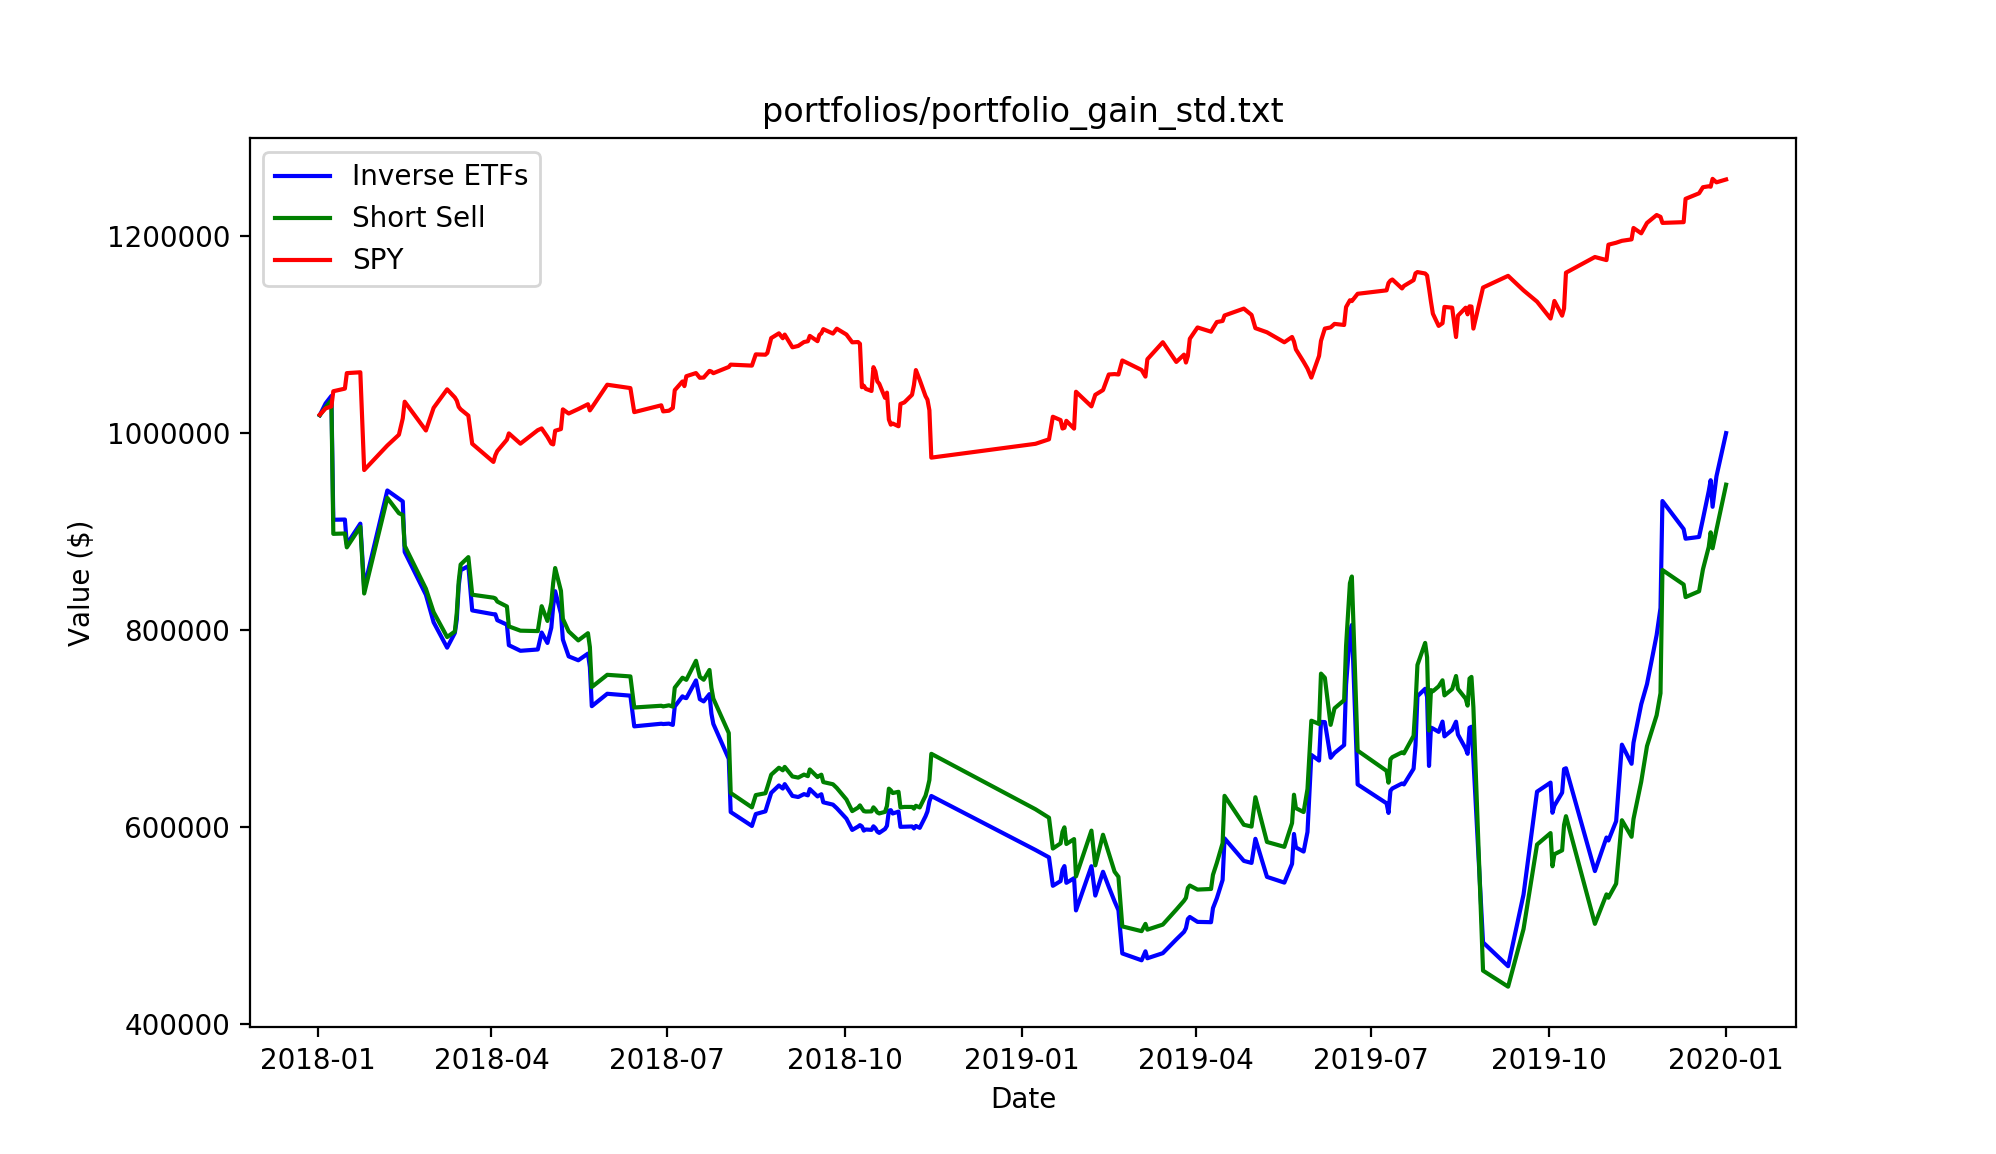
\includegraphics[scale=0.42,bb=0 0 320 240]{figures/Gain_std_maximization.png}
\caption{Results of ETF trading backtest using approach I; portfolio
  gain to standard deviation ratio.}
\label{fig:etf-results-approach-1}
\end{figure}

\section{Approach II: Historical Return and MAD}\label{section:approach-2}

Given the rather inaccurate short term predictions of the geometric
model, we use an alternative approach. The proposed algorithm is as
follows,

\begin{itemize}

  \item[1] At a given current time $t_{0}$ abuild a geometric forecast
    model using historical data, using $n$ economic variables,
    includng prices of the $\tilde{n}$ ETFs which are used as an asset
    pool for trading.

  \item[2] Given a trading horizon end time $t_{H} > t_{0}$, get the
    expected trends of the $\tilde{n}$ ETFs. This is the only piece of
    information we get from the geometric model. We only need to know
    whether price of an asset is expected to increase or decrease over
    a trading horizon. We can combine the trend predictions from the
    geometric model with a ''fall back'' method, as described in
    section~\ref{subsection:fallback-macd}, to increase the chance of
    a correct price trend forecast.

    \item[3] Calculate the historical mean and mean absolute deviation
      (MAD) of logarithmic return, and choose a subset of
      $\tilde{n}^{\prime}$ < $\tilde{n}$ which have the highet mean to
      MAD ratio. The logarithmic return for asset $i$ is calculated
      as,

      \begin{equation}\label{eqn:log-return}
        R^{i}(t) = \sum_{i=1}^{\tilde{n}}
        \frac{log(\hat{y}^{i}(t))-log(\hat{y}^{i}(t-1))}{log(\hat{y}^{i}(t-1))}
      \end{equation}

      The mean of $R^{i}$ is calculated as,

      \begin{equation}\label{eqn:log-return-mean}
        \bar{R}^{i} = \frac{1}{N} \sum_{k=-N}^{0} R^{i}(t_{k})
      \end{equation}

      where the last $N$ discrete times prior to $t_{0}$ are used to
      calculate the mean. SImilary, the MAD is calculated as,
      
      \begin{equation}\label{eqn:log-return-mad}
        MAD(R^{i}) = \frac{1}{N} \sum_{k=-N}^{0} |R^{i}(t_{k}) - \bar{R}^{i}|
      \end{equation}
      
  \item[4] Give each of the $\tilde{n}^{\prime}$ assets an equal
    weight in portfolio. If the proce is oredicted to increase take a
    long position, and if it is predicted to decrease take a short
    position.

   \item[5] Adjust the portfolio at $t_{H}$ by repeat the above steps;
     more generally, adjust the portfolio every $t_{H}$ - $t_{0}$.
      
\end{itemize}

\subsection{A Fallback Plan for Trend Prediction}\label{subsection:fallback-macd}

It is advised to keep a short out-of-sample period with available
historical data for each forecast model. We can then test the
performance of the model's trend prediction for each asset. If a model
fails to predict the correct trend of a security price in the
out-of-sample period following the training period, it will likely
fail beyond the out-of-sample period as well. In this case, we can
fall back on one of the more standard trend prediction
methodologies. As an example, we can use Moving Average Convergence
Divergence (MACD) method.

MACD is used to calculate short term acceleration of a security and as
such helps with making a decision to take a long or short position on
a security. MACD of a signal $x(t)$ is defined as,

\begin{equation}\label{eqn:macd}
F_{MACD}^{(f,s)}(x)|_{t_{0}} = E^{f}(x)|_{t_{0}} -
E^{s}(x)|_{t_{0}}
\end{equation}

where $E^{p}$ represents exponential moving average with respect to a
period $p$, and $f$ and $s$ are fast and slow periods,
respectively. The signal $x(t)$ has a positive/negative acceleration
at $t=t_{0}$ if $F_{MACD}^{(f,s)}(x)|_{t_{0}}$ is
greater/smaller than $E^{r}(F_{MACD}^{(f,s)}(x))|_{t_{0}}$, where
$r$ is called the signal period. The standard values for fast, slow,
and signal periods are 12, 26, and 9 days, respectively. One should
long/short when acceleration becomes positive/negative. In fact, one
can check the sign of both $F_{MACD}^{(f,s)}(x)|_{t_{0}}$ and
$F_{MACD}^{(f,s)}(x)|_{t_{0}}-E^{r}(F_{MACD}^{(f,s)}(x))|_{t_{0}}$
as they represent velocity and acceleration signs, respectively. The
number of historical times used to calculate MACD should be at least
$s$ + $r$ ($N > s + r$).

\subsection{Some Backtest Results for Aprroach II}\label{subsection:fallback-macd}

The approach II was tested using a model with 34 variables, consisting
of 27 ETFs and 7 constineous futures
contracts. Figure~\ref{fig:etf-results-approach-2} should the results
for 2018 and 2019.

\begin{figure}
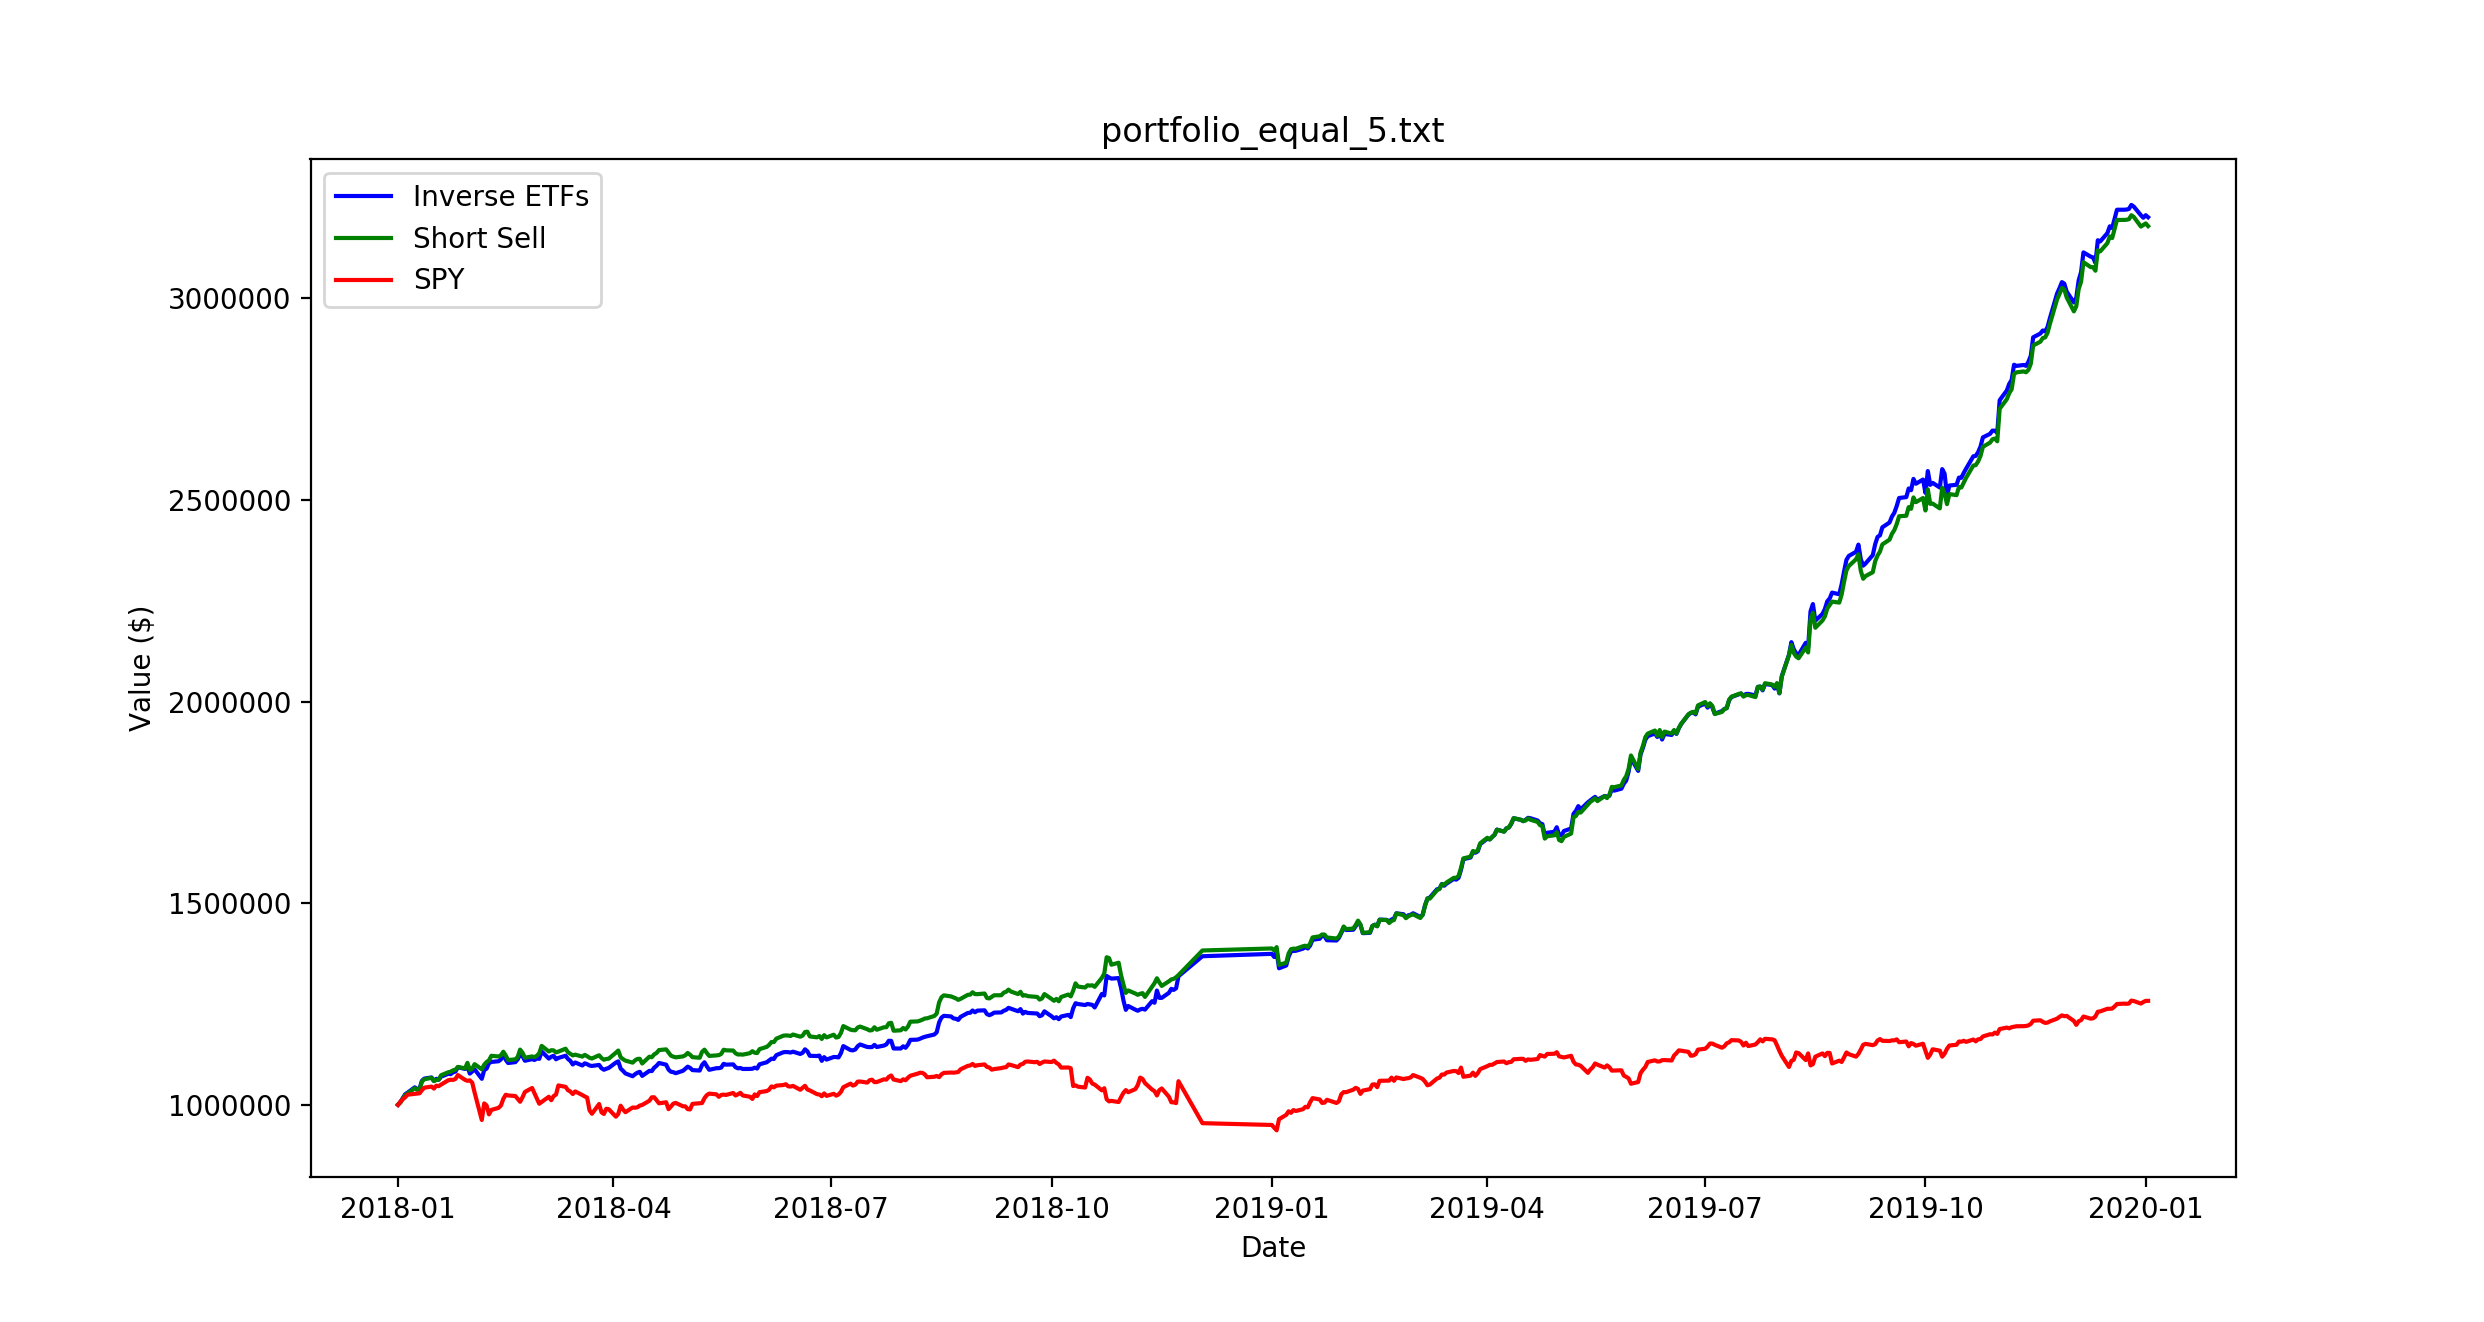
\includegraphics[scale=0.42,bb=0 0 320 240]{figures/sorted-5-Equal-60-days-eval.png}
\caption{Results of ETF trading backtest using approach II; here we
  used the geometric model qualitatively, only to predict the trends.}
\label{fig:etf-results-approach-2}
\end{figure}

\end{document}

